\documentclass[12pt]{article}

\usepackage[spanish, es-tabla]{babel}
\usepackage[utf8]{inputenc}
\usepackage[T1]{fontenc}
\usepackage{bookman}

\usepackage{amsmath, amsfonts, amssymb}

\usepackage[left=2.5cm, right=2.5cm, top=1.5cm]{geometry}

\usepackage{graphicx}
\usepackage{float}

\usepackage[nottoc,numbib]{tocbibind}
\usepackage{cite}

\title{Jerarquía de Chomsky}
\date{}


\begin{document}
	\maketitle
	\begin{center}
		Ian Mendoza Jaimes\\
		2CM4\\
		Prof. Genaro Juárez Martínez\\
		Teoría Computacional\\
		25 de octubre de 2016\\
	\end{center}

\vspace{2em}
	Noam Chomsky, lingüista estadounidense nacido en 1928, profesor del Instituto de Tecnología de Massachussets (MIT). Ha publicado más de 70 libros y más de 1000 artículos sobre diversos temas como lingüística, filosofía y política. Se le considerada el fundador de la Gramática generativa transformacional. 

En 1956 Chomsky publica "Three models for the description of language", un trabajo en el que se describen las propiedades de los tipos de lenguajes formales y correspondientes gramáticas en relación a su complejidad computacional. Según Chomsky, los tipos de lenguajes formales pueden dividirse en tres: de estados finitos (o regulares), de estructura de frase (o libres de contexto) y transformaciones (o sensibles al contexto). Tal clasificación es conocida como la jeraquía de Chomsky.

El principal objetivo de Chomsky y su jerarquía era demostrar que los dos primeros tipos de gramaticas son incapaces de dar cuenta, de manera simple y general, de la complejidad de las lenguas naturales. En particular, Chomsky demostró que el inglés presenta propiedades que no pueden ser reflejadas ni por gramáticas de estados finitos ni por gramáticas de estructura de frase.

\vspace{1em}

\begin{figure}[H]
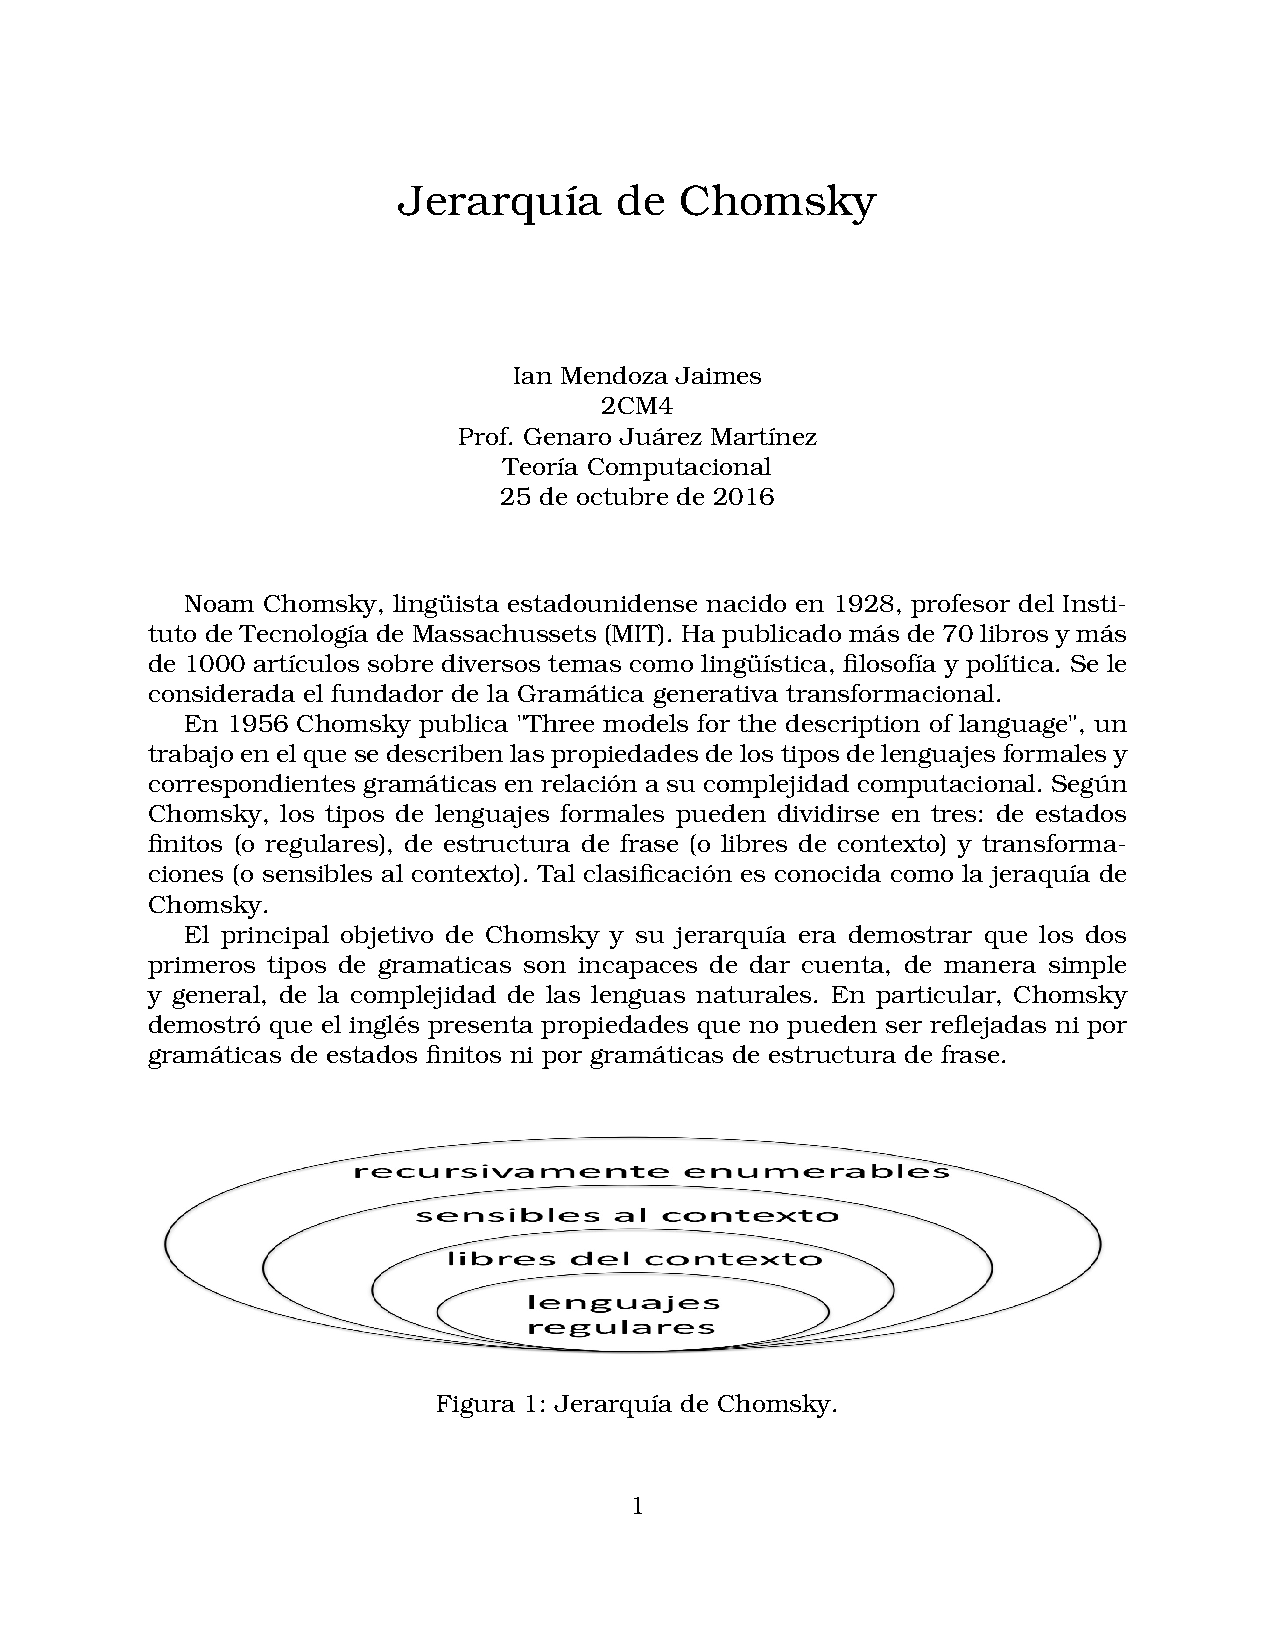
\includegraphics[width=\textwidth, height=4cm]{jerarquia}
\caption{Jerarquía de Chomsky.}
\label{fig:jerarquia}
\end{figure}

\vspace{1em}

La Figura 1 muestra un resumen de su jerarquia, a continuación será descrita mas detalladamente:

\begin{enumerate}

\item \textbf{Tipo 0, Lenguajes recursivos:} Es un lenguaje formal para el cual existe una máquina de Turing que acepta y se detiene con cualquier cadena del lenguaje. Pero que puede parar y rechazar, o bien iterar indefinidamente, con una cadena que no pertenece al lenguaje, en contraposición a los lenguajes recursivos en cuyo caso se requiere que la máquina de Turing pare en todos los casos.

\item \textbf{Tipo 1, Lenguajes sensibles al contexto:} Computacionalmente, un lenguaje sensible al contexto es equivalente a una máquina de Turing no determinista linealmente acotada, también llamado Autómata linealmente acotado. Se trata de una máquina de Turing no determinista con una cinta de sólo kn posiciones, donde n es el tamaño de la entrada y k es la constante asociada a la máquina. Esto significa que cada lenguaje formal que puede ser decidido por una máquina es un lenguaje sensible al contexto.

\item \textbf{Tipo 2, Lenguajes libres de contexto:} Están formados por gramáticas libres de contexto. En lingüística e informática, una gramática libre de contexto (o de contexto libre) es una gramática formal en la que cada regla de producción es de la forma: $V \longrightarrow w$, 
donde V es un símbolo no terminal y w es una cadena de terminales y/o no terminales. El término libre de contexto se refiere al hecho de que el no terminal V puede siempre ser sustituido por w sin tener en cuenta el contexto en el que ocurra. Un lenguaje formal es libre de contexto si hay una gramática libre de contexto que lo genera.

\item \textbf{Tipo 3, Lenguajes regulares}: Los lenguajes más sencillos que se considerarán son los lenguajes regulares, es decir, los que se pueden generar a partir de los lenguajes básicos, con la aplicación de las operaciones de unión, concatenación y * de Kleene un número finito de veces.

\end{enumerate}


\bibliographystyle{acm}
\bibliography{bibliografia}



\end{document}